
	\section{Terminology and concepts}

    \begin{frame}{Terminology and concepts}
        \begin{tikzpicture}
        \node[] at (-7, -3.25) {};
        \node[] at (7, 3.25) {};

        \node[anchor=west, inner sep=0pt, draw=black, label=below:\tiny{ChatGPT}] at (-7, 0) {
            \includegraphics[width=3.9cm]{data/chatgpt.png}
        };
        \node[inner sep=0pt, draw=black, label=below:\tiny{Spot}] at (-1, 1.3) {
            \includegraphics[width=2.5cm]{data/spot.jpg}
        };
        \node[inner sep=0pt, draw=black, label=below:\tiny{1X Neo}] at (2.2, 2.1) {
            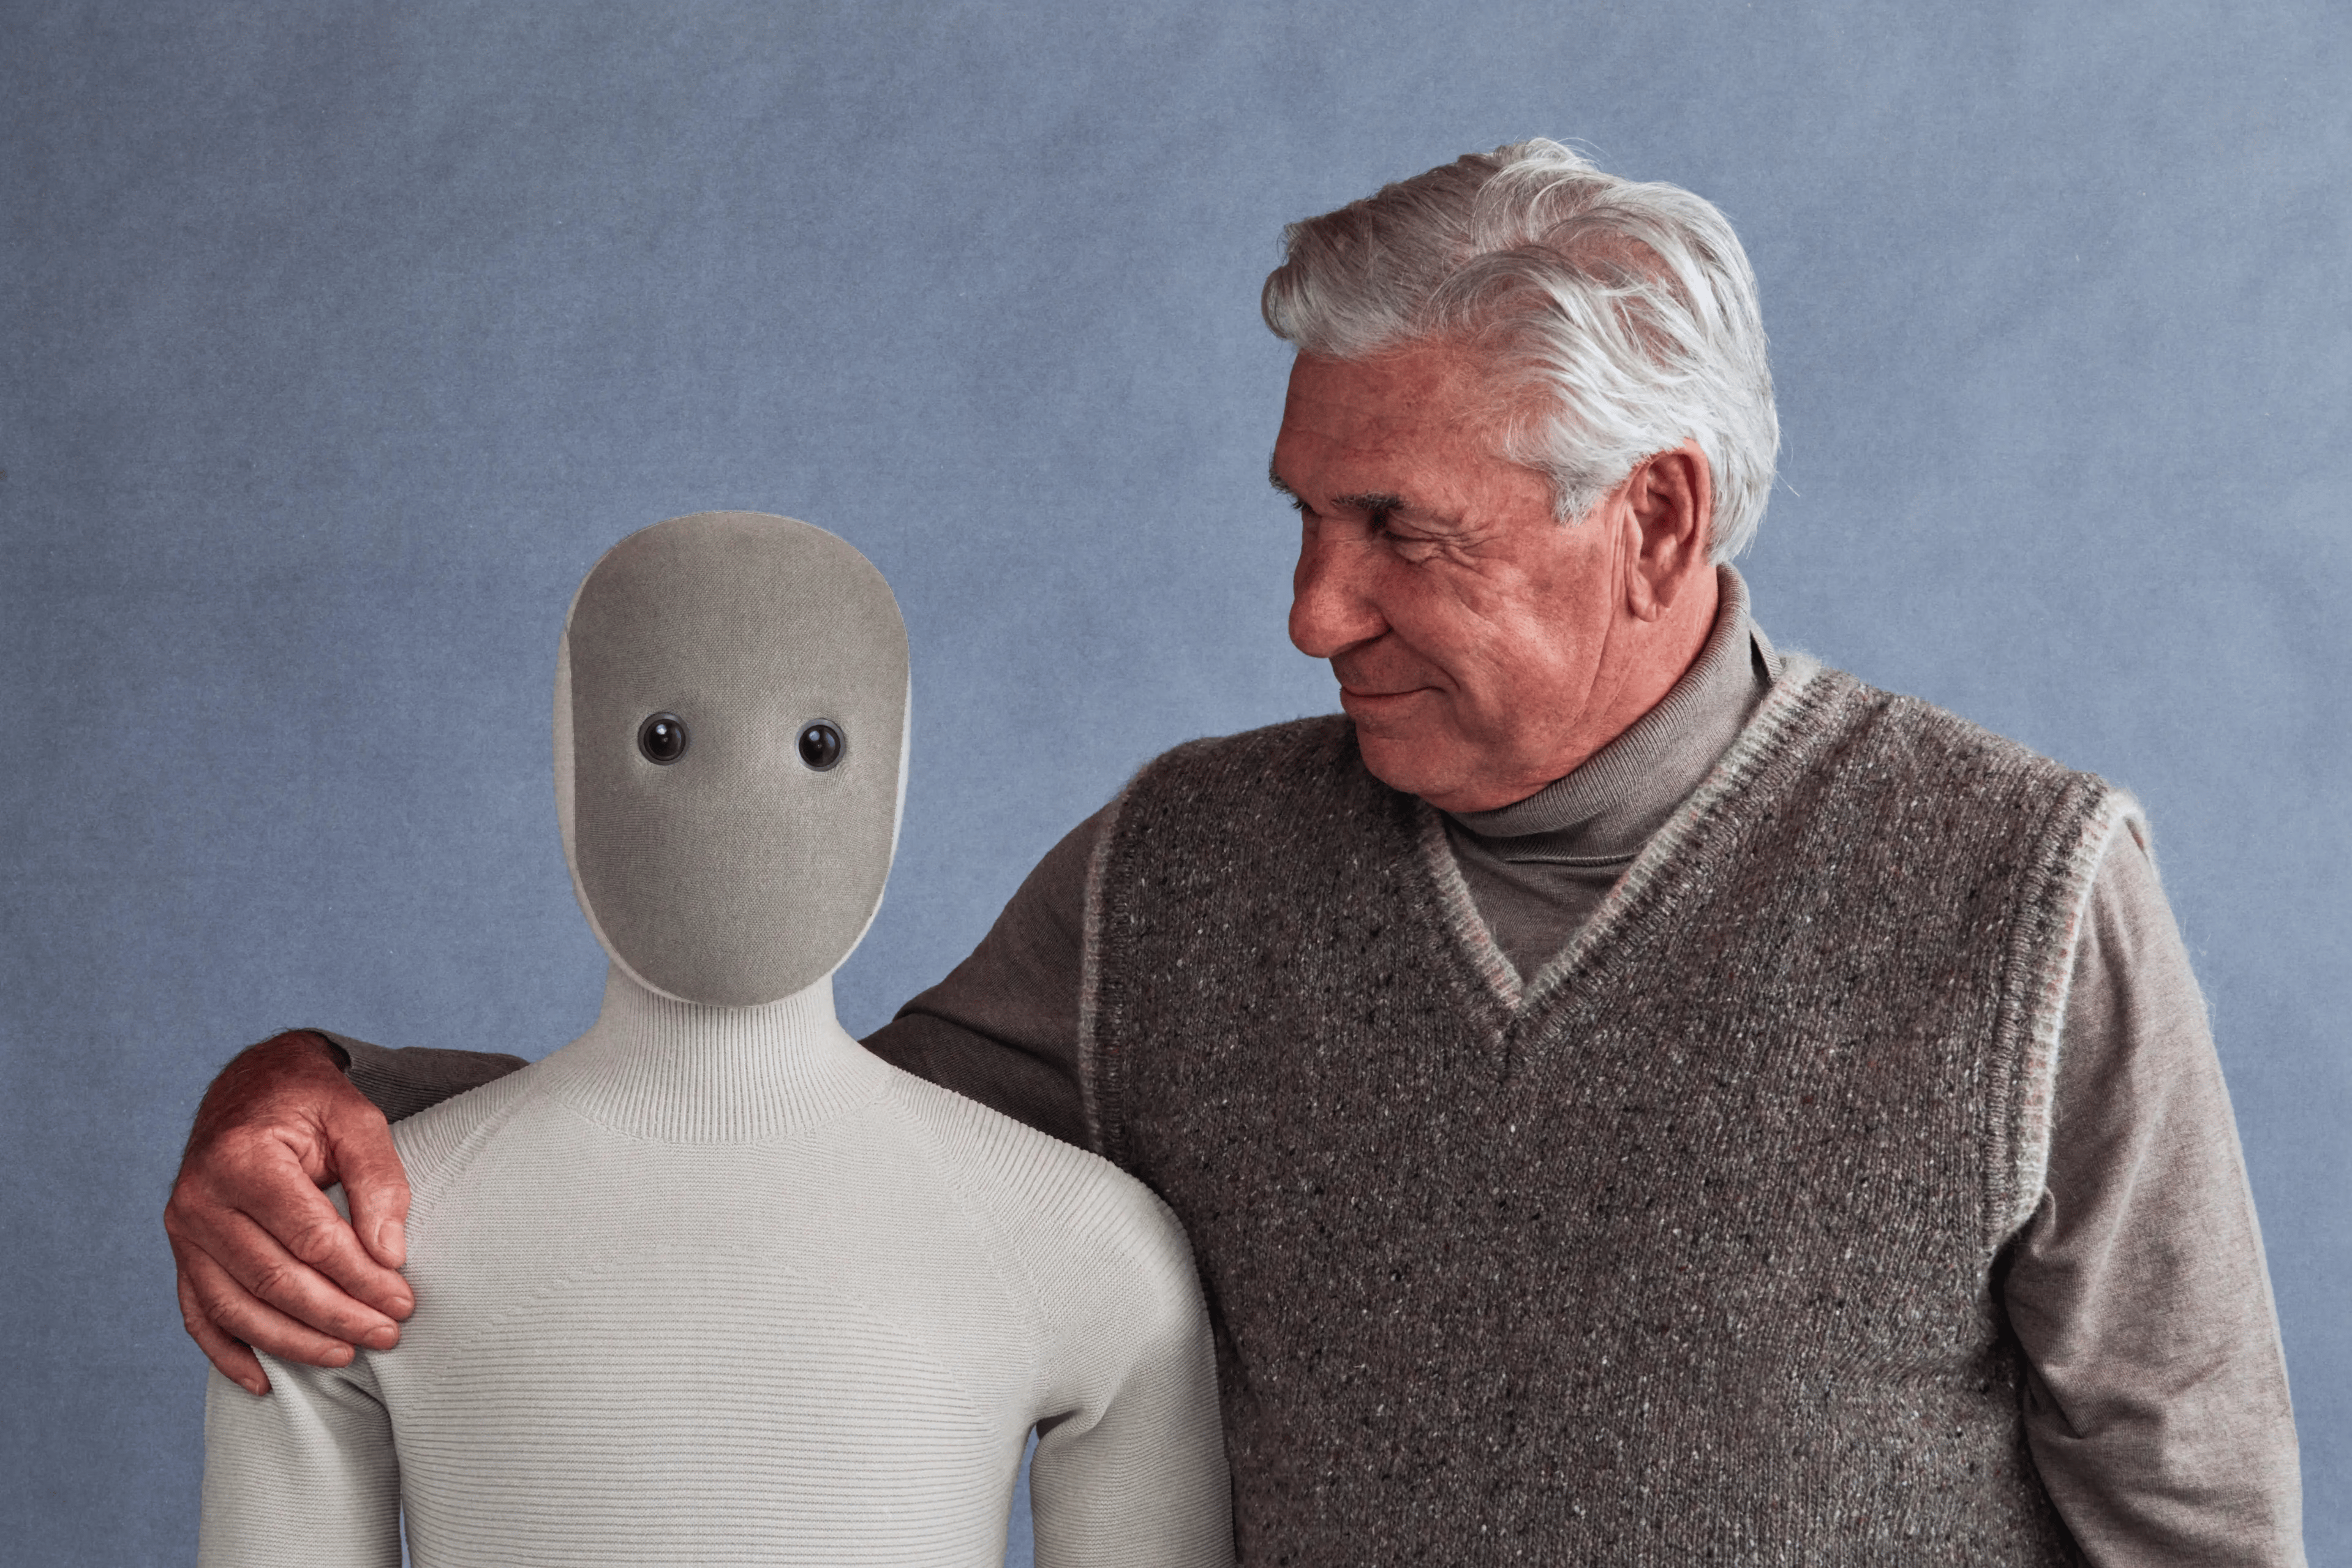
\includegraphics[width=2.5cm]{data/neo.png}
        };
        \node[inner sep=0pt, draw=black, label=below:\tiny{AlphaFold}] at (-1.1, -1.8) {
            \includegraphics[width=3cm]{data/alphafold.png}
        };
        \node[inner sep=0pt, draw=black, label=below:\tiny{AlphaZero}] at (2.4, -1.1) {
            \includegraphics[width=2.7cm]{data/chess.png}
        };

        \end{tikzpicture}
    \end{frame}

	\begin{frame}{Terminology and concepts: Taxonomy}
		\centering
		\vfill
		\begin{tikzpicture}
			\node[circle, fill=blue!60, minimum size=6cm] (ai) at (0, 0) {};
			\node[text=white, anchor=north] at ($ (ai.north) - (0, 0.3) $) {\textbf{Artificial intelligence}};

            \node[
                anchor=north west,
                align=left,
                font=\small,
                text width=4cm,
                alt=<1-4>{text=black}{text=gray!40}
            ] (ai-text) at ($ (ai.north) + (3.5, 0.2) $) {
                \only<1>{%
                    \textbf{Artificial intelligence:}\\Machines that solve tasks requiring some kind of (often human-like) intelligence.
                }%
                \only<2>{%
                    \textbf{Artificial intelligence:}\\Machines that solve a wide array of tasks in various environments.
                }%
                \only<3->{%
                    \textbf{Artificial intelligence:}\\The field that produces machines that solve a wide array of tasks in various environments.
                }%
            };

			\only<4->{
				\node[text=white] at ($ (ai.north) - (-1.1, 1.2) $) {Symbolic AI};
			}
			\only<5->{
				\node[circle, fill=purple!60, minimum size=4.5cm, anchor=south] (ml) at ($ (ai.south) + (0, 0.05) $) {};
				\node[text=white, anchor=north] at ($ (ml.north) - (0, 0.3) $) {\textbf{Machine learning}};

				\node[
                    anchor=north west,
                    align=left,
                    font=\small,
                    text width=4cm,
                    alt=<5-6>{text=black}{text=gray!40}
                ] (ml-text) at ($ (ai-text.south west) - (0, 0) $) {\textbf{Machine learning:}\\Machines that learn to solve tasks by learning patterns from data};
			}
			\only<6->{
				\node[text=white, align=center, font=\linespread{0.5}\selectfont] at ($ (ml.north) - (1, 1.1) $) {Linear\\regression};
			}
			\only<7->{
				\node[circle, fill=red!60, minimum size=3cm, anchor=south] (dl) at ($ (ai.south) + (0, 0.1) $) {};
				\node[text=white, anchor=north] at ($ (dl.north) - (0, 0.3) $) {\textbf{Deep learning}};

				\node[
                    anchor=north west,
                    align=left,
                    font=\small,
                    text width=4cm,
                    alt=<7>{text=black}{text=gray!40}
                ] (dl-text) at ($ (ml-text.south west) - (0, 0) $) {\textbf{Deep learning:}\\Machine learning models organized in hierarchies ($\approx$ deep neural networks) inspired by the brain};
			}
			\only<8>{
				\node[align=center, text=white, font=\linespread{0.5}\selectfont] at ($ (dl.north) - (-0.2, 1.2) $) {Convolutional\\neural networks};
				\node[align=center, text=white, font=\linespread{0.5}\selectfont] at ($ (dl.north) - (0.2, 2.1) $) {Large language\\models};

				\node[
                    anchor=north west,
                    align=left,
                    font=\small,
                    text width=4cm
                ] (cnn-text) at ($ (dl-text.south west) - (0, 0) $) {
                    \textbf{Convolutional neural nets:}\\Neural networks for image data
                };
				\node[
                    anchor=north west,
                    align=left,
                    font=\small,
                    text width=4cm
                ] at ($ (cnn-text.south west) - (0, 0) $) {
                    \textbf{Large language models:}\\Neural networks for natural language (e.g. ChatGPT)
                };
			}
		\end{tikzpicture}
		\vfill
	\end{frame}

	\begin{frame}{Terminology: Supervision}
		\centering
		\vfill
		\begin{tikzpicture}
			\node[align=center, anchor=north] (supervised) at (0, 0) {Supervised learning};
			\node[align=center, anchor=north] (unsupervised) at (7, 0) {Unsupervised learning};
			\draw[] (3.5, 0) -- (3.5, -7.5);
			\node[] (cat1) at ($ (supervised.south) + (-1, -0.8) $) {
				\includegraphics[width=1.2cm]{data/cat.1.jpg}
			};
			\node[anchor=west] (cattext1) at ($ (cat1.east) + (1.2, 0) $) {Cat};
			\draw[->] (cat1) -- (cattext1);
			\node[anchor=north] (dog1) at ($ (cat1.south) + (0, -0.1) $) {
				\includegraphics[width=1.2cm]{data/dog.0.jpg}
			};
			\node[anchor=west] (dogtext1) at ($ (dog1.east) + (1.2, 0) $) {Dog};
			\draw[->] (dog1) -- (dogtext1);
			\node[anchor=north] (cat2) at ($ (dog1.south) + (0, -0.1) $) {
				\includegraphics[width=1.2cm]{data/cat.2.jpg}
			};
			\node[anchor=west] (cattext2) at ($ (cat2.east) + (1.2, 0) $) {Cat};
			\draw[->] (cat2) -- (cattext2);
			\node[anchor=north] (dog2) at ($ (cat2.south) + (0, -0.1) $) {
				\includegraphics[width=1.2cm]{data/dog.1.jpg}
			};
			\node[anchor=west] (dogtext2) at ($ (dog2.east) + (1.2, 0) $) {Dog};
			\draw[->] (dog2) -- (dogtext2);

			\node[] (cat1) at ($ (unsupervised.south) + (-1.2, -1.9) $) {
				\includegraphics[width=0.8cm]{data/cat.1.jpg}
			};
			\node[] (cat2) at ($ (cat1) + (-0.9, 0.2) $) {
				\includegraphics[width=0.8cm]{data/cat.2.jpg}
			};
			\node[] (cat3) at ($ (cat1) + (-0.5, -0.8) $) {
				\includegraphics[width=0.8cm]{data/cat.3.jpg}
			};
			\node[] (cat4) at ($ (cat1) + (0.9, -0.1) $) {
				\includegraphics[width=0.8cm]{data/cat.4.jpg}
			};

			\node[] (dog1) at ($ (cat1) + (1.8, -2.5) $) {
				\includegraphics[width=0.8cm]{data/dog.0.jpg}
			};
			\node[] (dog2) at ($ (dog1) + (0.9, 0.1) $) {
				\includegraphics[width=0.8cm]{data/dog.1.jpg}
			};
			\node[] (dog3) at ($ (dog1) + (0.3, -0.8) $) {
				\includegraphics[width=0.8cm]{data/dog.3.jpg}
			};
			\node[] (dog4) at ($ (dog1) + (-0.9, -0.3) $) {
				\includegraphics[width=0.8cm]{data/dog.4.jpg}
			};
		\end{tikzpicture}
		\vfill
	\end{frame}

	\begin{frame}{Terminology: Strong and weak AI}
		\centering
		\vfill
		\begin{tikzpicture}
			\draw[<->] (0, 0) -- (10, 0);
			\node[anchor=north west] at (0, -0.1) {More specific};
			\node[anchor=north east] at (10, -0.1) {More general};
			\node[anchor=north west] at (0, 6) {Narrow (weak)};
			\node[anchor=north east] at (10, 6) {General (strong)};

			\draw[red, ->, thick] (2, 4) -- (8, 4);
			\node[anchor=south,align=center,text=red] at (5, 4.1) {Able to solve a broader spectrum of\\problems in a wider array of domains};

			\visible<2->{
				\node[anchor=south east] at (9.5, 0.2) {
					\includegraphics[width=1.3cm]{data/human.png}
				};
				\node[anchor=south west] at (0.5, 0.2) {
					\includegraphics[width=1.3cm]{data/laptop.png}
				};
			}
			\visible<3->{
				\node[align=center,font=\small, fill=blue!60, text=white, minimum width=1.6cm, rounded corners=.1cm] at (3, 2.1) {
					Image\\
					diagnostics
				};
				\node[align=center,font=\small, fill=blue!60, text=white, minimum width=1.6cm, rounded corners=.1cm] at (3, 1.3) {
					Insurance\\
					pricing
				};
				\node[align=center,font=\small, fill=blue!60, text=white, minimum width=1.6cm, rounded corners=.1cm] at (3, 0.5) {
					Document\\
					reading
				};
			}
			\visible<4>{
				\node[align=center,font=\small, fill=blue!60, text=white, minimum width=1.6cm, rounded corners=.1cm] at (4.8, 0.5) {
					Tesla
				};
				\node[align=center,font=\small, fill=blue!60, text=white, minimum width=1.6cm, rounded corners=.1cm] at (5.4, 1.1) {
					ChatGPT
				};
			}
		\end{tikzpicture}
		\vfill
	\end{frame}